\chapter{Homolog\'ia Persistente}

La homolog\'ia persistente es una herramienta poderosa que es usada para el computo, estudio y codificaci\'on
multiescala de propiedades topol\'ogicas de familias anidadas de complejos simpliciales y espacios
topol\'ogicos. No solo provee algoritmos eficientes para calcular los n\'umeros de Betti de cada complejo
en las familias consideradas, como se requiere para la inferencia homol\'ogica cubierta en la secci\'on
anterior, sino que tambi\'en codifica la evoluci\'on de los grupos de homolog\'ia de los
complejos anidados a trav\'es de las escalas. Ideas y resultados preliminares que culminan en la
teor\'ia de la homolog\'ia persistente pueden ser encontrados desde antes del siglo XXI, en particular
en los trabajos de Barannikov (1994) \cite{Barannikov1994}, Frosini (1992) \cite{Frosini1992},
Robins (1999) \cite{Robins1999}; pero su desarrollo en su forma moderna se concreto en los trabajos
de Edelsbrunner et al. (2002) \cite{Edelsbrunner2002} y Zomorodian y Carlsson (2005)
\cite{Zomorodian2005}.

\section{Filtraciones}

Una filtraci\'on de un complejo simplicial $K$ es una familia anidada de subcomplejos
$\cpar{K_{r}}_{r\in t}$, donde $T\subseteq\mathbb{R}$, tal que para cualquier
$r, r' \in T$, si $r\leq r'$ entonces $K_{r}\subseteq K_{r'}$ y $K = \bigcup_{r\in T}K_{r}$.
El subconjunto $T$ puede ser finito o infinito. En general, una filtraci\'on de un espacio
topol\'ogico $\mathbb{M}$ es una familia anidada de subespacios $\cpar{M_{r}}_{r\in T}$,
donde $T\subseteq\mathbb{R}$, tal que para cualquier $r, r' \in T$,
si $r\leq r'$ entonces $M_{r}\subseteq M_{r'}$ y $M = \bigcup_{r\in T}M_{r}$. Por ejemplo, si
$f: \mathbb{M}\rightarrow\mathbb{R}$ es una funci\'on, entonces la familia
$M_{r} = f^{-1}\cpar{\left(-\infty, r\right]}$, $r\in\mathbb{R}$ define una filtraci\'on llamada la
filtraci\'on del conjunto subnivel de $f$.

En la pr\'actica, el par\'ametro $r\in T$ suele ser interpretado como un par\'ametro de escala, y las
filtraciones com\'unmente usadas en el ATD suelen pertenecer a uno de los siguientes dos tipos.

\section*{Filtraciones Sobre Datos}

Dado un subconjunto $\mathbb{X}$ de un espacio m\'etrico compacto $\cpar{M,\rho}$, las familias de
complejos de Vietoris-Rips $\cpar{Rips_{r}\cpar{\mathbb{X}}}_{r\in\mathbb{R}}$ y los complejos de \v Cech
$\cpar{Cech_{r}\cpar{\mathbb{X}}}_{r\in\mathbb{R}}$ son filtraciones\footnote{Aqu\'i consideramos
$Rips_{r}\cpar{\mathbb{X}} = Cech_{r}\cpar{\mathbb{X}} = \varnothing$, si $r<0$}. Aqu\'i, el par\'ametro
$r$ puede ser interpretado como la resoluci\'on con la que se considera el conjunto de datos $\mathbb{X}$.
Por ejemplo, si $\mathbb{X}$, es una nube de puntos en $\mathbb{R}^{d}$, gracias al teorema del nervio,
la filtraci\'on $\cpar{Cech_{r}\cpar{\mathbb{X}}}_{r\in\mathbb{X}}$ codifica la topolog\'ia de todo la
familia de uniones de bolas $\mathbb{X}^{r} = \cup_{x\in\mathbb{X}}B\cpar{x,r}$, cuando $0<r<\infty$.
Como la noci\'on de filtraci\'on es algo flexible, se han considerado muchas otras filtraciones en la
literatura para ser construidas sobre los datos, como el complejo testigo popularizado en el ATD por
De Silva y Carlsson (2004)\cite{DeSilva2004}, las filtraciones de Rips con peso Buchet et al.
(2015)\cite{Buchet2015b}, o las filtraciones DTM Anai et al. (2019)\cite{Anai2019} que nos permiten
trabajar con conjuntos de datos con ruido o con datos at\'ipicos.

\section*{Filtraciones de Conjuntos Subnivel}

Definir funciones en los v\'ertices de un complejo simplicial da lugar a otro importante ejemplo de
filtraci\'on: sea $K$ el complejo simplicial con el conjunto de v\'ertices $V$ y
$f:V\rightarrow\mathbb{R}$. Entonces $f$ puede ser extendida a todos los simplices de $K$ definiendo
$f\cpar{\ccorch{v_{0},\dots,v_{k}}} = \max\cllav{f\cpar{v_{i}}: i=1,\dots,k}$ para cualquier simplejo
$\sigma = \ccorch{v_{0},\dots,v_{k}}\in K$ y la familia de subcomplejos,
$K_{r}=\cllav{\sigma\in K:f\cpar{\sigma}\leq r}$, define una filtraci\'on llamada la filtraci'on del
conjunto subnivel de $f$. La filtraci\'on del conjunto sobre-nivel de $f$ se define de manera similar.

En la pr\'actica, incluso si el \'indice del conjunto es infinito, todas las filtraciones consideradas
son construidas en conjuntos finitos y son, en si, finitas. Por ejemplo, cuando $\mathbb{X}$ es finito,
el complejo de Vietoris-Rips $Rips_{r}\cpar{\mathbb{X}}$ cambia solo en un numero finito de \'indices,
$r$. Esto nos permite manejarlos de manera sencilla desde una perspectiva algebraica.

\section{Algunos Ejemplos}

Dada una filtraci\'on $\mathit{Filt} = \cpar{F_{r}}_{r\in T}$ de un complejo simplicial o un espacio
topol\'ogico, la homolog\'ia de $F_{r}$ cambia cuando $r$ incrementa; pueden aparecen nuevos componentes
conexos y algunos ya existentes pueden unirse, aros y cavidades pueden formarse o llenarse, etc. La
homolog\'ia persistente registra estos cambios, identifica las propiedades que aparecen y asocia un
tiempo de vida a cada una. La informaci\'on resultante se codifica como un conjunto de intervalos llamado
c\'odigo de barras, o bien, como un conjunto de puntos en $\mathbb{R}^{2}$ donde la coordenada de
cada punto es el punto de inicio y final de cada intervalo correspondiente.

Antes de dar una definici\'on formal, ilustraremos el concepto de homolog\'ia persistente con unos
ejemplos.

% IDE Change, change to hard-wrapping per sentence instead of hard-wrapping per max number of char.

\section*{Ejemplo 1}

Sea $f:\ccorch{0,1}\rightarrow\mathbb{R}$ la funci\'on de la Figura \ref{fig:Figura 9},
y sea $F_{r} = f^{-1}\cpar{\cpar{-\infty,r}}_{r\in\mathbb{R}}$ la filtraci\'on del conjunto subnivel de $f$.
Todos los conjuntos subnivel de $f$ son o bien vacios o la uni\'on de intervalos,
as\'i que la \'unica informaci\'on topol\'ogica no-trivial que brindan es su homolog\'ia cero dimensional, esto es, su n\'umero de componenetes conexas.
Para $r<a_{1}$, $F_{r}$ es vacio, pero para $r = a_{1}$, aparecen un primer componente conexo en $F_{a_{1}}$.
La homolog\'ia persistente registra $a_{1}$ como la ``fecha de nacimiento'' de una componente conexa la codifica como un intervalo que comienza en $a_{1}$.
Luego, $F_{r}$ permanece conexo hasta que $r$ toma el valor de $a_{2}$ donde una segunda componente conexa aparece.
La homolog\'ia persitente registra esta nueva componente conexa creando un segundo intervalo que comienza en $a_{2}$.
De manera similar, cuando $r$ alcanza el valor de $a_{3}$, una nueva componente conexa aparece y la homolog\'ia persistente crea otro intervalo comenzando en $a_{3}$.
Cuando $r$ alcanza $a_{4}$, las dos componentes creadas en $a_{1}$ y $a_{3}$ se juntan para crear una sola componente conexa.
En este paso, la homolog\'ia persistente sigue la regla de que la componente que muere es la m\'as reciente que ha aparecido en la filtraci\'on;
As\'i, el intervalo que comenz\'o en $a_{3}$ termina en $a_{4}$,
y el intervalo de persistencia que codifica el tiempo de vida de la componente nacida en $a_{3}$ es creado.
Cuando $r$ alcanza $a_{5}$, como en el caso previo la componente nacida en $a_{2}$ muere y se crea el intervalo $\cpar{a_{2},a_{5}}$.
El intervalo creado en $a_{1}$ permanece hasta el final de la filtraci\'on,
dando lugar al intervalo $\cpar{a_{1},a_{6}}$ si la filtraci\'on se detiene en $a_{6}$,
o bien, $\cpar{a_{1},\infty}$ si $r$ tiende a $+\infty$ (en cuyo caso la filtraci\'on se mantiene constante para $r>a_{6}$).
El conjunto de intervalos obtenidos que codifican el tiempo de vida de diferentes caracteristicas homol\'ogicas a lo largo de la filtrac\'on es llamado el codigo de barras de persistenca de $f$.
Cada intervalo $\cpar{a,a'}$ puede ser representado en el plano $\mathbb{R}^{2}$ por el punto $\cpar{a,a'}$.
El conjunto de puntos resultante es llamado el diagrama de persistencia de $f$.
Es de notar que la funci\'on puede tener multiples copias del mismo intervalo en su codigo de barras de persitencia.
Como consecuencia, el diagrama de persistenca de $f$ es un multiconjunto donde cada punto tiene una multiplicidad entera asociada.
Finalmente, por razones t\'ecnicas que seran claras m\'as adelante,
se a\~{n}aden al diagrama de persistencia todos los puntos de la diagonal $\Delta = \cllav{\cpar{b,d}: b=d}$ con multiplicidad infinita.

\begin{figure}[ht]
    \centering
    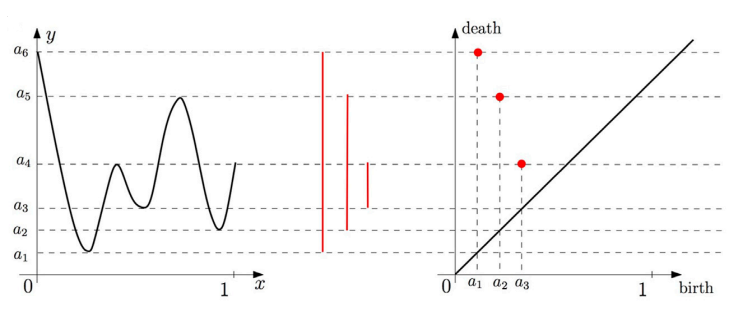
\includegraphics[width=0.85\linewidth]{./figures/Figura9.png}
    \caption{
        El c\'odigo de barras de persistencia y el diagrama de persistencia de la funci\'on
        $f:\ccorch{0,1}\rightarrow\mathbb{R}$.
    }
    \label{fig:Figura 9}
    \vspace{15pt}
\end{figure}

\section*{Ejemplo 2}

Sea $f: M\rightarrow \mathbb{R}$ la funci\'on eb la Figura \ref{fig:Figura 10},
donde $M$ es una superficie de dos dimensiones homeomorfa a un toro,
y sea $F_{r} = f^{-1}\cpar{\cpar{-\infty,r}}_{r\in \mathbb{R}}$ la filtraci\'on del conjunto subnivel de $f$.
La homolog\'ia persistente cero dimensional se calcula como en el ejemplo anterior,
lo cual genera las barras rojas en el codigo de barras de persistencia.
En este caso los subniveles tambi\'en almacenan informaci\'on acerca de caracter\'isticas homol\'ogicas uno dimensionales.
Cuando $r$ alcanza la altura $a_{1}$,
los conjuntos subnivel $F_{r}$ que eran homeomorfos a dos discos se vuelven homeomorfos a la uni\'on disjunta de un disco y un \'anulo,
creando un primer ciclo homologo a $\sigma_{1}$ en la Figura \ref{fig:Figura 10}.
El nacimiento de este uno-ciclo es representado por un intervalo (en azul) que comienza en $a_{1}$.
Similarmente, cuando $r$ alcanza $a_{2}$, un segundo ciclo, homologo a $\sigma_{2}$, es creado,
dando lugar al comienzo de un nuevo intervalo de persistencia.
Estos dos ciclos nunca son rellenos (abarcan $H_{1}\cpar{M}$) de manera que los intervalos que les corresponden continuan por el resto de la filtraci\'on.
Cuando $r$ alcanza $a_{3}$, un nuevo ciclo es creado, el cual se rellena en $a_{4}$,
lo cual genera el intervalo de persistencia $\cpar{a_{3},a_{4}}$.
Esta vez, la filtraci\'on del conjunto subnivel da lugar a dos codigos de barras,
uno par la homolog\'ia cero dimensional (mostrado en rojo) y otro para la homolog\'ia uno dimensional (mostrado en azul).
Estos dos codigos de barras pueden ser representados de manera equivalente como diagramas en el plano. 

\begin{figure}[ht]
    \centering
    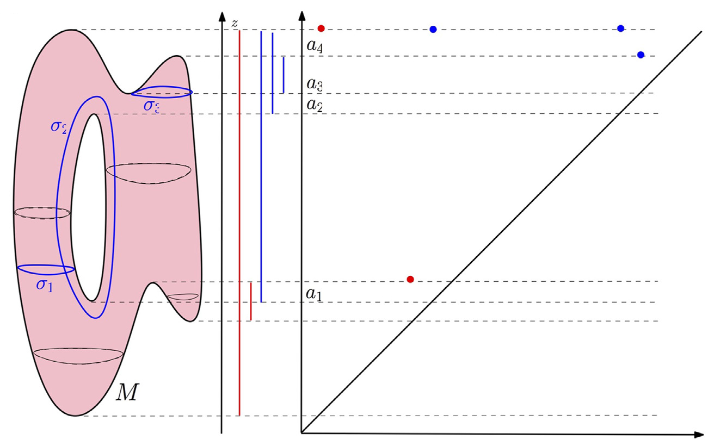
\includegraphics[width=0.85\linewidth]{./figures/Figura10.png}
    \caption{
        El codigo de barras de persistencia y el diagrama de persistencia de la funci\'on altura
        (proyecci\'on en el eje $z$) definida en una superficie en $\mathbb{R}^{3}$.
    }
    \label{fig:Figura 10}
    \vspace{15pt}
\end{figure}

\section*{Ejemplo 3}

En este \'ultimo, consideramos la filtraci\'on dada por la uni\'on de bolas
(que crecen linealmente)
centradas en el conjunto de puntos finitos $C$ en la Figura \ref{fig:Figura 11}.
Notese que esta es la filtraci\'on del conjunto subnivel de la funci\'on distancia a $C$,
y gracias al teorema del nervio,
esta filtraci\'on es homot\'opicamente equivalente a la filtraci\'on de \v Cech construida sobre $C$.
La Figura \ref{fig:Figura 11} muestra varios conjuntos subnivel de la filtraci\'on de la siguiente manera:

\begin{enumerate}[label=\alph*)]
    \item Para radio $r=0$, la uni\'on de bolas se reduce al conjunto de puntos finito inicial,
    cada uno de ellos correspondiendo a una componente conexa;
    se comienza un intervalo por cada una de estas componentes en $r=0$.

    \item Algunas de las bolas comienzan a superponerse,
    resultando en la muerte de algunas de las componentes conexas que se han juntando entre s\'i;
    el diagrama de persistencia registra estas muertes, poniendo fin a los intervalos correspondientes.
    
    \item M\'as componentes conexas se han juntado, dejando una sola componente conexa,
    y as\'i, todos los intervalos asociados a caracter\'isticas cero dimensionales terminan,
    con la excepci\'on de los que corresponden a las componentes restantes;
    dos nuevas caracter\'isticas uno dimensionales han aparecido,
    lo cual resulta en dos nuevos intervalos (en azul) que comienzan en ese valor de $r$.
    
    \item Una de los dos ciclos uno dimensionales se ha rellenado,
    resultando en su muerte en la filtraci\'on y en el fin del intervalo correspondiente.
    
    \item Todas la componenetes uno dimensionales han muerto, dejando un \'unico intervalo rojo en el codigo de barras.
    como en ejemplos anteriores, el codigo de barras puede ser representado como un diagrama de persistencia,
    donde cada intervalo $\cpar{a,b}$ es representa por un punto en $\mathbb{R}^{2}$ de coordenadas correspondientes.
    
\end{enumerate}

Intuitivamente afirmamos que entre m\'as largo sea un intervalo en el codigo de barras,
o bien, equivalentemente,
entre m\'as alejado est\'e un punto de la diagonal en el diagrama correspondiente,
m\'as persistente, y por tanto, relevante, es la propiedad homol\'ogica que le corresponde a trav\'es de la filtraci\'on.
Es de notar tambi\'en que para un radio $r$ dado, el $k$.-\'esimo n\'umero de Betti de la uni\'on de bolas en cuesti\'on,
es igual al n\'umero de intervalos de persistencia correspondiendo a caracter\'isticas homol\'ogicas $k$ dimensionales que contienen a $r$.
As\'i, el diagrama de persistencia puede ser visto como una firma topol\'ogica que codifica la homolo\'gia de la uni\'on de bolas abiertas,
para todos los radios, as\'i como su evoluci\'on a trav\'es de los valores que toma $r$.

\begin{figure}[ht]
    \centering
    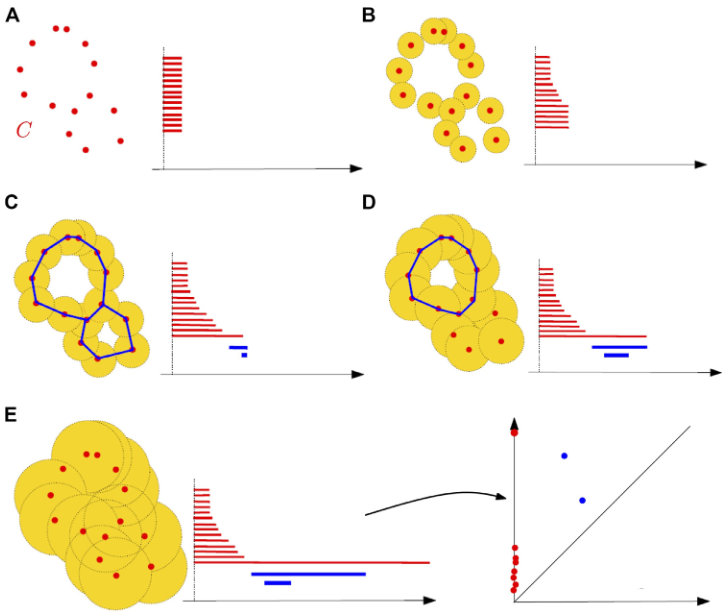
\includegraphics[width=0.85\linewidth]{./figures/Figura11.png}
    % \caption{
    %     Placeholder
    % }
    \label{fig:Figura 11}
    \vspace{15pt}
\end{figure}

\newpage

\section{Modulos y Diagramas de Persistencia}

Inicia nueva secci\'on.